% !TEX root = ../main.tex

\section{Asymmetric cryptography}
\label{Async}
Asymmetric cryptography\footnote{Often also referred to as Public-key cryptography.} is a term used to describe crypto-systems that use key pairs rather than a common shared secret - as in symmetric cryptography. The key pair consists of a private key, only known to the owner of the key pair, and a public key that is visible to the public.

Asymmetric cryptography covers more than simply encryption and decryption. Key generation can also be done asymmetrically with schemes such as the Diffie-Hellman key exchange. This sort of asymmetric cryptography will not be a focus in this paper, as encryption/decryption is the main focus.

There is, however, a third use for asymmetric cryptography, which will become interesting when all of this is done reversibly: digital signatures. With the private key being known only to the owner, anything that can be successfully decrypted with the public key can therefore only have been sent by them.
\subsection{RSA}
\label{RSA}
RSA is an asymmetric cryptosystem developed in the 1970s by Ron \textbf{R}ivest, Adi \textbf{S}hamir, and Leonard \textbf{A}dleman, and is arguably the best known and most commonly used cryptography algorithm\cite{RSA}. It implements the public/private key pair infrastructure used in asymmetric cryptography and uses integer factorization to provide security.

\subsubsection{Integer Factorization}
The algorithm makes use of the integer factorization problem which deals with the decomposition of a composite number\cite{integerfactor}. It is well known to be significantly harder to find the factor of a product, than calculating the product of two integers. The RSA algorithm, therefore, assumes that it is computationally expensive to solve the prime factorization problem given a large composite \textit{n}, such that $n=p \cdot q$ where $p\neq q$ and $p$ and $q$ are both prime\cite{RSA}. This essentially works as a one-way trap door function, which is easy to compute in one direction, but almost impossible to perform in the reverse direction. An example of this can be seen below:
$$n = p \cdot q = 44560482149 \cdot 6620830889=295027416640832300461$$


%This \textit{n} might be rather trivial to factorize for a computer, and it is therefore important to choose sufficiently large prime numbers, to generate a large enough \textit{n}. This \textit{n} will be used as the modulus for both the private and public keys as well as for key-generation. Hence the National Institute of Standards and Technology suggests a bit-length of at least 2048 to provide adequate security\cite{RecommendationForKeyManagement}. 

This value of \textit{n} might be rather trivial to factorize for a computer, and it is, therefore, important to choose sufficiently large prime numbers, to generate a large enough \textit{n}. This \textit{n} will be used as the modulus for both the private and public keys as well as key-generation in the cryptographic stage of the algorithm. Hence the National Institute of Standards and Technology suggests a bit-length of at least 2048 to provide adequate security \cite{RecommendationForKeyManagement}. 

% https://nvlpubs.nist.gov/nistpubs/SpecialPublications/NIST.SP.800-57Pt3r1.pdf

% n used in key generation? Er det egentlig det? Det er jo faktisk phi af n som man bruger til at generere krypterings exponenten



% the fundamental theorem of arithmetic, every positive integer has a unique prime factorization.

%%%%%%%%%%%%%%%%%%%%%%%%%%%%%%%%%%%%%%%%%%%%%%%%%%%%%%%%%%%%%%%%%%%%%%%%%%%%
%%% Danny freestyler lige lidt, det er ikke nødvendigvis noget der skal med i rapporten.
\subsubsection*{Modular exponentiation}
The goal of this project is only encryption/decryption (no key generation), which in RSA essentially boils down to modular exponentiation. A promising method for implementing modular exponentiation (specifically considering Hermes), is a left-to-right binary method. The reason this method is more appealing than others is the looping over binary representations. Since looping is rather restricted in Hermes, this is a good method for looping, while staying within the boundaries of Hermes. A more in-depth look at this method will be provided in Chapter \ref{OurRSA}. 

%Recall from section \ref{Hermes}, that Hermes is restricted in several ways, to eliminate time-based side-channel attacks. These restrictions become somewhat troublesome when attempting to implement exponentiation, as execution time for exponentiation is very much dependent on the exponent. As RSA implementations are, omitting key generation, simply modular exponentiation, this is a bit of a bump in the road. To get around this, it is necessary to investigate different approaches to modular exponentiation.
%%% Talk a bit about Exponentiation by squaring and left-to-right binary method. More about the one that turns out to work, if any! 
%%%%%%%%%%%%%%%%%%%%%%%%%%%%%%%%%%%%%%%%%%%%%%%%%%%%%%%%%%%%%%%%%%%%%%%%%%%%

%>>>>>>>>>>>>>>>>Head
%\subsubsection{Public key cryptosystem}
%The private key \textit{d} and a public key \textit{e} are defined has two keys used to decrypt and encrypt messages when communicating. The couple ($N,e$) constitutes the public key, where $n=p \cdot q$ is the modulus and $e$ the encryption exponent. However, \textit{e} cannot be picked randomly and must therefore obey the following properties:
%=================
\subsubsection{RSA discrete logarithm problem}
Commonly referred to as the RSA problem\cite{RSAProblem}, it refers to the infeasibility of computing $m$ in $C=m^e ~ (mod ~ n)$ given the RSA public key $(n,e)$ and the ciphertext $C$, for a sufficiently large $n$. Given that it is trivial to compute in one direction, and practically impossible to do in reserve, is known as a one-way trapdoor function. This is closely related to the integer factorization problem and is together the basis of security for the RSA encryption scheme . 


\subsubsection{Public/Private key cryptosystem}
The private key \textit{(d,n)} and a public key \textit{(e,n)} are used to decrypt and encrypt respectively. The pair ($N,e$) constitutes the public key, where $n=p \cdot q$ is the modulus and $e$ the encryption exponent. However, \textit{e} cannot be picked randomly and must therefore obey the following properties: 
\[e=\begin{Bmatrix}
1 < e < \phi (n)   \\
e \bot N, \phi (n)
\end{Bmatrix}
\]
Where $\phi (N) = (p-1)(q-1)$.

When encrypting a message using RSA, a message \textit{m} must first be converted to integers using a binary translation.% To perform the encryption step, both parties must first exchange their public keys (\textit{N,e}).
The sender of the message can now apply the receiver's public key to encrypt the message \textit{m} into ciphertext \textit{c} using the following formula:

$$c \equiv m^{e}(mod ~ N)$$

After having performed this step, the sender is now able to communicate the ciphertext \textit{c} to the correspondent. Recovering the original message from \textit{c} requires the use of the private key $(N,d)$.% The decryption exponent \textit{d} is derived by taking modular multiplicative inverse of $e ~ (mod ~ \phi (N))$, which is straightforward since information about $\phi (N) = (p-1)(q-1)$ is known to the owner of the public and private key.
The receiver of the message now recover the plaintext \textit{m} by computing:


%Reverting the ciphertext \textit{c} back into the original message $m$ requires the use of the private key $(N,d)$. The decryption exponent \textit{d} is derived by taking modular multiplicative inverse of $e ~ (mod ~ \phi (N))$, which is straightforward since information about $\phi (N) = (p-1)(q-1)$ is known to the owner of the public and private key. The receiver of the message now recover the plaintext \textit{m} by computing:

$$c^d ~(mod ~~ N)\equiv (m^e)^d ~(mod ~~ N)\equiv m^{ed} ~(mod ~~ N)\equiv m^{N \phi(N)+1} ~(mod ~~ N)\equiv M$$

\newpage

\subsection{Elliptic curve cryptography}
\label{elliptic}
Elliptic curve cryptography (ECC) is another asymmetric cryptosystem. The curve itself is a function on the form $E: ~ y^2 \equiv x^3+ax+b $ also called a Weierstrass curve, where $a$ and $b$ are the parameters of the curve\cite{elipticcurve}. The shape of the curve changes with these parameters. %%%%%%%
%ECC uses the same underlying principles as other public key cryptosystems of the form $g^a ~ mod ~n$, where \textit{g} is the generator, \textit{a} is the secret exponent and \textit{n} is the modulus $n \in \mathbb{P}$. However, in ECC this is done over an elliptic curve structure.
\begin{figure}[H]
    \centering
    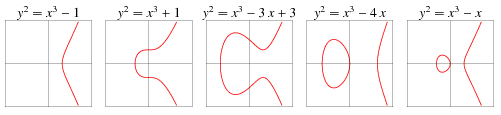
\includegraphics[width=1.0\textwidth]{figures/elliptic-curve-example}
    \caption{Example shapes of elliptic curves given different parameters $a,b$ in the form  $E: ~ y^2 \equiv x^3+ax+b $}
\end{figure}
\noindent This structure can be defined by the equation:
$$\{(x,y) \in \mathbb{R}^{2} ~ | ~ y^2 \equiv x^3 +ax +b, 4a^3 + 27b^2 \not\equiv 0 \} \cup \{0\}$$
where $4a^3+27b^2 \neq 0$ to avoid singular points.

The geometry of elliptic curves allows for adding points together. This point-addition is not the same as regular arithmetic addition, but shares some properties with it, hence the name. 
\subsubsection{Elliptic Curve Point-Addition}
\label{ECPA}
Adition on an elliptic curve is not an actual arithmetic operation, but rather a geometrical one. It is done by drawing a line through the two points, which will intersect the curve at a third point $R'$. Reflecting this new point $R'$ on the x-axis results in yet another point on the curve, called $R$.

$$P \oplus Q = R$$

For this operation to properly inherit the properties of arithmetic addition, an additive identity is necessary. This is what is referred to as the point-at-infinity, and is denoted $\mathcal{O}$. This point is the result of any addition which draws a perfectly vertical line through the two points\cite{IntroToMath}. 
%\mathcal{O}

The addition law on an elliptic curve \textit{E} can now be described as:\\
\begin{figure}[H]

\textbf{Theorem 6.5}. \textit{Let E be an elliptic curve. Then the addition law on E has the following properties:}\\
(a) $~~~~~ P + \mathcal{O} = \mathcal{O} + P = P ~~~~~~~~~~~~~~~ for ~ all ~~ P \in E. ~~~~~~~~~ [\text{Identity}]$ \\
(b) $~~~~~ P + (-P) = \mathcal{O} ~~~~~~~~~~~~~~~~~~~~~~ for ~ all ~~ P \in E. ~~~~~~~~~~ [\text{Inverse}]$ \\
(c) $~~~~ (P+Q) + R = P+(Q+R) ~~~~~ for ~ all ~~ P,Q,R \in E. ~~~ [\text{Assosiative}]$ \\
(d) $~~~~~~ P + Q = Q+P ~~~~~~~~~~~~~~~~~~~~ for ~ all ~~ P,Q \in E. ~~~~~~~~ [\text{Commutative}]$ 
\caption{Theorem 6.5: Addition law on elliptic curves\cite{IntroToMath}.}
\end{figure}


Notice how the theorem refers to a negation of a point ($-P$). This negation can be understood as flipping the point over the curve, and so if $P=\{x,y\}$ then $-P=\{x,-y\}$.

\begin{figure}[H]
    \centering
    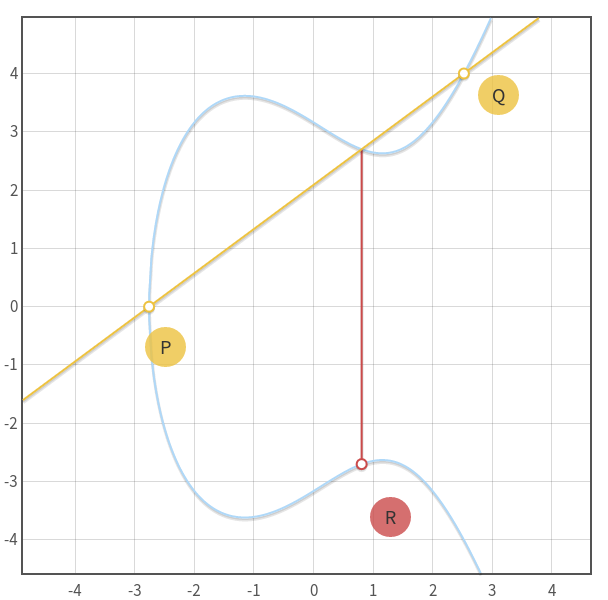
\includegraphics[width=0.7\textwidth]{figures/ECC-point-addition}
    \caption{Illustrating Point addition over the elliptic curve $y^2 = x^3 - 4x + 10$ in $\mathbb{R}$ where $P = (-2.76082, 0)$, $Q = (2.5251, 5)$ and $R = (0.80836, -2.70089)$.}
\end{figure}

\noindent The coordinates of a point $R = P\oplus Q$ are defined as:
\[R_x:= \lambda^2-P_x-Q_x\]
\[R_y:= -P_y+\lambda(P_x-R_x)\]
Where $\lambda$ is defined as:
\[\lambda := \frac{P_y-Q_y}{P_x-Q_x}\]

\subsubsection{Point-Doubling}
A special case of point addition is that in which the two points have the same coordinates: $P={x,y}=Q$. This case is referred to as point doubling and is done slightly differently than the addition of two distinct points.

To double a point, the line that is followed is the tangent at the point $P$. If $P_y \neq 0$, then this tangent line will intercept the curve at another point $R'$, and flipping the point over the $x$-axis yields the result $R$.

If, on the other hand, $P_y = 0$ then $R=2P = \mathcal{O}$, as the tangent in such a point will be vertical. 

\noindent The coordinates of the point $R=2P$ are defined similarly to simple addition:
\[R_x:= \lambda^2-2P_x\]
\[R_y:= -P_y+\lambda(P_x-R_x)\]
except for the calculations for finding $\lambda$:
\[\lambda := \frac{3*P_x^2+a}{2P_y}\]
where $a$ is $a$-coefficient from the curve.

\subsubsection{Point-Multiplication}
With a point-addition defined, repeatedly adding a point to itself is called point-multiplication (just like multiplication is defined in regular arithmetics). That is, a point $P$ multiplied by a number $n$ is defined as:
$$nP = \underbrace{P\oplus P\oplus P\oplus \ldots \oplus P}_\text{n copies}$$
This operation is the core of elliptic curve cryptography (ECC), in both key generation and encryption/decryption.

For any curve used in ECC, points for multiplication are not chosen at random. Instead a generator point $G$ is chosen for a curve, which can then be added to itself any number of times.

\subsubsection{Elliptic curve discrete logarithm problem}
Having multiplied a point $G$ by some number $n$, yielding a new number, is a process that is computationally infeasible to retrace. Given a curve $E$ and the points $G, Q \in E$, one would have to find an integer \textit{n}, if it exists, such that $Q = nG$. This is known as the “elliptic curve discrete logarithm problem” (ECDLP)\cite{elipticcurve}\cite{logarithmproblem}.
% WierStrass Form: https://crypto.stanford.edu/pbc/notes/elliptic/weier.html


\subsubsection{Elliptic Curve over Finite Fields}
Elliptic curve arithmetics over a real number plane $(x,y) \in \mathbb{R}$ is often used to exemplify the computational steps in the arithmetics. However, ECC is typically done over a predefined finite field.

When limiting the points from $\mathbb{R}$ to ${\mathbb{F}_p}$ or ${\mathbb{F}_p}^2$ the curve is then defined by:
$$\{(x,y) \in \mathbb{F}_{p} ~ | ~ y^2 \equiv x^3 +ax +b ~ (mod ~ p), 4a^3 + 27b^2 \not\equiv 0 ~ (mod ~ p) \} \cup \{0\}$$
Here $x,y$ are constant values from a finite field $\mathbb{F}_{p}$, where p is a prime number that determines the size of the field\cite{elipticcurvefinite}. Not only must coordinates be within the field, but the same goes for the coefficients of the curve: $a,b\in\mathbb{F}_p$.

Addition and multiplication are performed in the same manner, except all computations are performed $mod~p$.

This representation means that the curve no longer looks the same, as it is now a seemingly scattered group of points. There is, however, still symmetry in the points, as the curve has, in a sense, simply been shifted up above the $x$-axis. 
%The point $P$ specifies a predetermined base point also called the generator point $G=(x_P, y_P)$ on the curve and \textit{n} is a prime of the order of $P$ which initially determines the maximum value that can be turned into a private key.

\begin{figure}[H]
    \centering
    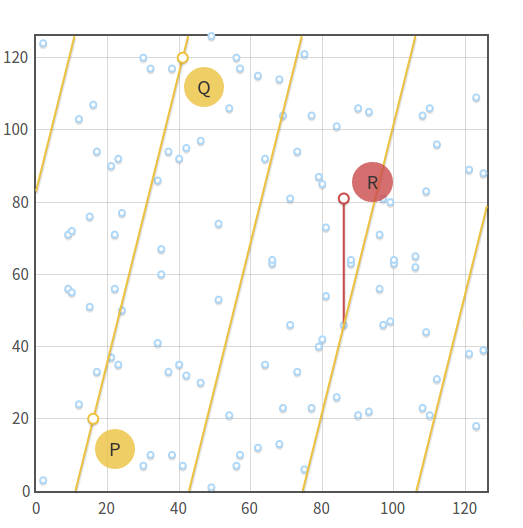
\includegraphics[width=0.6\textwidth]{figures/ECC-finite-field}
    \caption{Example of point addition over the curve $y^2 = x^3-x+3$ in $\mathbb{F}_{127}$ with $P = (16, 20)$, $Q = (41, 120)$ and $R = (86, 81)$}
\end{figure}

Not all curves are pleasant to work with, and proving properties about them is a difficult process. NIST has published a collection of suggested curves over a variety of Finite Fields (both prime fields, as described here, but also extension fields, more on that in Section \ref{Galois}).
\subsubsection{Elliptic Curve Integrated Encryption Scheme (ECIES)}
For an elliptic curve $E$ on the form $y^2=x^3+ax+b$ over a prime field $\mathbb{F}_p$, the encryption is rather elegant\footnote{https://asecuritysite.com/encryption/ecc3}. With some generator point, $G$, for the curve, a person (say Alice, the usual suspect) can produce a public/private key-pair by choosing a random number $d$ and multiplying that with the generator point $G$: $dG=Q$. The new point $Q$ is the public key, and the random number $d$ is the private key. 

When a sender (say Bob, Alice's ages-old friend) wants to encrypt a message for Alice, he does the following:
\begin{enumerate}
\item Chooses a random number $r$.
\item Generates 2 new points: $S=rQ$ and $R=rG$.
\item Derives a key from the point $S$ using an arbitrary Key Derivation Function (KDF) and symmetrically encrypts his message using that key.
\item Sends his encrypted message, as well as the point $R$ to Alice.
\end{enumerate}
Alice can now decrypt the message by:
\begin{enumerate}
\item Computing the point $S$ by multiplying the point $R$ sent to her by Bob with her private key $d$.
\item Deriving a key from the point $S$ using the same Key Derivation Function (KDF).
\item Symmetrically decrypting the message with the key.
\end{enumerate}
To see why this works, consider:
\[S=rQ=rdG=drG=dR\]
This holds due to the properties of point-addition described in Section \ref{ECPA}. 
\newpage

%%%% UNUSED/REWRITTEN STUFF %%%%

%================================================================================
%\noindent This point addition is now repeated by drawing a line through \textit{P} and \textit{R'}, thus intersection with a new point \textit{Q} on the curve. Again, we find the inverse of this point and repeat the same operation. 


%However, instead of adding two arbitrary points, we use a specific base point \textit{P} on the curve which will be added together.


%The same operation is used to add and reflect the point across the x-axis. however now we just continuously add \textit{P} together, thus computing $nP$. For a point \textit{P} on the elliptic curve and a non-negative scalar \textit{n}, we now define $nP$ to be:
%$$nP = \underbrace{P+P+P+ \ldots + P}_\text{n copies}$$

%<<<<<<< HEAD
%Performing this operation \textit{n} times will yield a final point $Q = nP$. These elements will be used as keys in the cryptosystem, due to the infeasibility of findiæng \textit{n} even though you have the starting point \textit{P} and some ending point \textit{Q}. ECC, therefore, exploits the difficulty of computing the discrete logarithm of a random elliptic curve element for a publicly known base point, or the “elliptic curve discrete logarithm problem” (ECDLP)\cite{elipticcurve}. 
%=======
%This repeated addition is called point multiplication. Performing this operation \textit{n} times will yield a final point $Q = nP$. These elements will be used as keys in the cryptosystem, due to the infeasibility of finding \textit{n} even though you have the starting point \textit{P} and some ending point \textit{Q}. ECC, therefore, exploits the difficulty of computing the discrete logarithm of a random elliptic curve element for a publicly known base point, or the “elliptic curve discrete logarithm problem” (ECDLP)\cite{elipticcurve}. 


%\subsubsection{Point at infinity}
%Recall from theorem 6.5 in \ref{mylabel} how the identity element of an elliptic curve is defined for elliptic curve addition:
%\begin{align*}
%\mathcal{O} + P = P \\
%P + (-P) = \mathcal{O} 
%\end{align*}

%\noindent Both the identity and inverse law requires a point $\mathcal{O}$ to exist to be true. This point on the curve is defined as the identity element also called point at infinity and lies on all vertical lines and can be written as (0,0). 

%\textbf{Skal nedstående med?}\\
%Showing that for any point $P$ there exist an inverse is now a trivial task due to our point at infinity as we know that when reflecting the point at infinity $-\mathcal{O} = \mathcal{O}$, it yields the same point at infinity showing that an inversion is the same \textit{x-coordinate} but with an inverse \textit{y-coordinate} consequently showing that $P + (-P) = \mathcal{O}$\\
%\textbf{slutter her}
%\begin{figure}[H]
%    \centering
%    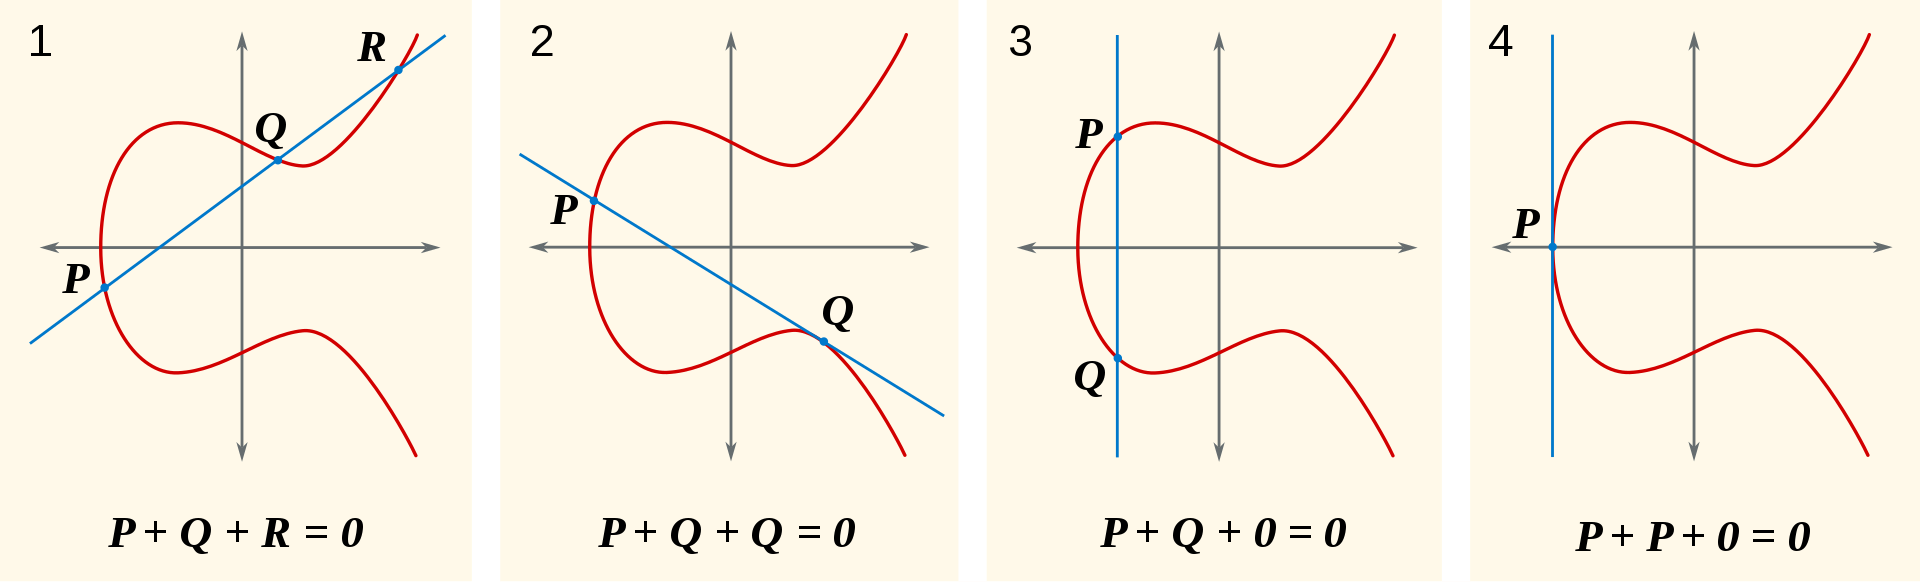
\includegraphics[width=1.0\linewidth]{figures/pointofinfinity}
%    \caption{Elliptic curve point operations: Addition (shown in facet 1), doubling (facets 2 and 4) and negation (facet 3).}
%    \label{fig:pointofinfinity}
%\end{figure}
%The ability to sum two points on the curve in simple Weierstrass form, which are each others' inverses, is not possible without the existence of point at infinity, because it would require the diversion of zero, which is not an allowed operation. This also means that the slope cannot be calculated because $P_x = Q_x$ as can be seen in facet 3 and 4 in figure \ref{fig:pointofinfinity}. Similar problem arises when trying to double a point $P_x = 0$. Hence the point at infinity is there to fill these gaps in the elliptic curve addition and acts as a neutral element (zero)\cite{IntroToMath}.
%>>>>>>> 893ba619fd33b3d23df071caa73202bb7cdfce33



% Question: Should the section below be either split up, rewritten, or placed elsewhere?






